\chapter{Implementierung}
\label{cha:implementierung}

In diesem Kapitel wird die Implementierung, genannt \emph{Ubermep}, des in Kapitel \ref{cha:entwurf} vorgestellten Architekturentwurfs erl"autert.

In Abschnitt \ref{sec:einleitung} wird zun"achst ein "Uberblick "uber die Struktur der Implementierung gegeben. Danach wird erl"autert wo und wie die im Grundlagenteil in Kapitel \ref{cha:grundlagen} 
vorgestellten Technologien Anwendung finden. Anschlie"send wird das im Entwurfskapitel spezifizierte Protokoll in Abschnitt \ref{sec:impl_protokoll} sowie die entwickelte Bibliothek, also der Kern der Implementierung in Abschnitt \ref{sec:ubermep-core} genauer beleuchtet.

In Abschnitt \ref{sec:beispiele} wird dann anhand von Beispielen gezeigt, wie ein Peer-to-Peer Overlay-Netzwerk mittels der Implementierung erzeugt werden kann. Weiter wird gezeigt wie man "uber das Netzwerk Nachrichten des Message Exchange Pattern versendet, sowie Remote Procedure Calls "uber das Netzwerk ausf"uhrt.

Abschlie"send wird in Abschnitt \ref{sec:zukunft} eine Auswahl von m"oglichen zuk"unftigen Erweiterung der Implementierung vorgestellt.

\section{Einleitung und "Uberblick}
\label{sec:einleitung}

Wie bereits in Abschnitt \ref{sec:maven} erl"autert, wurde diese Arbeit mittels dem Build-Tool Maven entworfen. Daraus ergibt sich eine Projektstruktur bestehend aus verschiedenen Maven-Untermodulen welche im Folgenden Abschnitt erl"autert werden. 
\subsection*{Struktur und Komponenten}

Diese Implementierung besteht aus 5 verschiedenen Untermodulen welche in einem sogenannten {\it Multi Module Project} zusammengefasst werden. Jedes Untermodul erbt von der Parent POM des {\bf Ubermep-parent} Moduls. Die Aufteilung der verschiedenen Module ist hierbei im Listing \ref{lst:ubermep-parent-dir} zu erkennen.

\lstinputlisting[language=Python,caption=Ausschnitt aus der Ubermep-parent pom.xml,label=lst:ubermep-parent-dir,firstnumber=1]{lst/ubermep-parent-dir.txt}

Im Folgenden nun eine kurze Beschreibung der einzelnen Module: 
\begin{itemize}
\item {\bf ubermep-parent} ist das Parent-Modul dieser Arbeit, welches den Parent-POM enth"alt. In seiner {\tt pom.xml} werden dabei die enthaltenen Untermodule, sowie die in den Untermodulen ben"otigten Abh"angigkeiten definiert. Diese Abh"angigkeiten werden dann an die Untermodule vererbt.
\item{\bf ubermep-cmdline} enth"alt den Einstiegspunkt zum starten der Applikation aus der Kommandozeile. 
\item{\bf ubermep-core} enth"alt die Bibliothek von ubermep. Dieses Modul h"alt unter anderem das zentrale Interface {\bf Peer} bereit, welches ben"otigt wird um ein Overlay-Netzwerk zu erzeugen und Nachrichten des Message Exchange Pattern auszutauschen. Dieses Modul wird in Abschnitt \ref{sec:ubermep-core} detailiert erkl"art.
\item{\bf ubermep-example} enth"alt Beispiel-Anwendungen wie ubermep-core genutzt werden kann. 
\item{\bf ubermep-gui} enth"alt eine grafische Oberfl"ache zum Erzeugen eines Over\-lay-Netzwerks sowie zum Senden von Nachrichten des Message Exchange Pattern.
\end{itemize}
Nur das Modul {\bf Ubermep-core} enth"alt die Bibliothek von ubermep und deshalb wird in diesem Kapitel, in Abschnitt \ref{sec:ubermep-core}, auch nur auf dieses Modul n"aher eingegangen. Im Folgenden aber zun"achst die Implementierung des in Abschnitt \ref{sec:protokoll} vorgestellten Protokolls.

% <----- START Protokoll

\section{Protokoll}
\label{sec:impl_protokoll}
Wie im Abschnitt \ref{sec:google-protobuf} bereits erl"autert, wird zum Generieren der Protokoll-Nachrichten Google-Proto\-buf verwendet. Im Listing \ref{lst:meppacket} ist die mittels der Proto\-buf-IDL erstellten Protokoll-Datei zu erkennen, die auf der Spezifikation des Protokoll-Entwurfs (\ref{sec:protokoll}) des Entwurfskapitel 3 basiert. Diese kann unter Benutzung des Protobuf-Compiler als serialisierte Protokoll-Nachricht "uber den Kommunikationskanal versendet werden.

\subsubsection{MEPPacket}
Das serialisierbare Protokoll dieser Applikation, das {\it MEPPacket}, ist wie folgt aufgebaut:

\lstset{caption=MEP.proto,label=lst:meppacket}
\begin{lstlisting}
message MEPPacket {
    required bool reliable = 1;
    required MessageType messageType = 2;
    required bytes payload = 3;
    
    optional uint32 requestID = 4;
    optional bool exceptionOccurred = 5;
    optional uint32 currentMessageNumber = 6;
    optional uint32 totalMessageNumber = 7;
    optional RPCMessage rpcMessage = 8;
}
\end{lstlisting} 

Es besteht aus den ben"otigten {\it (required)} Feldern: 
\begin{itemize}
\item {\bf reliable} spezifiziert ob eine Unicast bzw. Multicast-Nachricht {\it reliable} und {unreliable} ist. Request-Response-Nachrichten sind immer {\it reliable}.
\item {\bf messageType} beschreibt den Pattern - Typ der Nachricht. Eine genauere Beschreibung findet sich weiter unten.
\item {\bf payload} enth"alt den Inhalt einer Nachricht.
\end{itemize}
sowie den optionalen {\it (optional)} Feldern, die nur "ubertragen werden, wenn ben"otigt:
\begin{itemize}
\item {\bf requestID} wird intern f"ur die Abarbeitung von Request-Response-Nach\-rich\-ten ben"otigt. Jeder Request bekommt beim Aufruf eine RequestID zugewiesen. Wird die "uber die RequestID gekennzeichnete korrespondierende Response empfangen, so wird der Request als erfolgreich ausgeliefert gewertet.
\item {\bf exceptionOccured} zeigt an ob Server-seitig, also auf der Seite des Em\-pf"ang\-ers, beim Abarbeiten des {\it payloads} eine Ausnahme aufgetreten ist.
\item {\bf currentMessageNumber} zeigt an, welche Nummer die Antwort besitzt. Dieses Feld wird ausschlie"slich f"ur MultiResponse-Responses ben"otigt.
\item {\bf totalMessageNumber} zeigt an, wieviel Antworten versendet bzw. erwartet werden. Dieses Feld wird ausschlie"slich f"ur MultiResponse-Responses ben"otigt.
\item {\bf rpcMessage} beschreibt eine RPC-Message. Eine genauere Erl"auterung findet sich weiter unten.
\end{itemize}

\paragraph{MessageType}
Der Aufz"ahlungstyp {\it MessageType} spezifiziert den Pattern -Typ der Nachricht und ist wie folgt aufgebaut: 

\lstset{firstnumber=12, label=lst:messageType}
\begin{lstlisting}
enum MessageType {
    UNICAST = 1;
    MULTICAST = 2;
    SINGLE_RESPONSE_REQUEST = 3;
    MULTI_RESPONSE_REQUEST = 4;
    SINGLE_RESPONSE = 5;
    MULTI_RESPONSE = 6;
    RPC_REQUEST = 7;
    RPC_RESPONSE = 8;
}
\end{lstlisting}
Der MessageType enth"alt die folgenden Nachrichten-Typen:
\begin{itemize}
\item {\bf UNICAST} ist zust"andig f"ur Unicast Nachrichten; hierbei findet keine Unterscheidung zwischen unreliable bzw. reliable Unicast statt. Dies wird "uber das Flag {\bf reliable} im {\bf MEPPacket} spezifiziert.
\item {\bf MULTICAST} ist zust"andig f"ur Multicast Nachrichten; auch hierbei findet keine Unterscheidung zwischen unreliable bzw. reliable Multicast statt.
\item {\bf SINGLE\_RESPONSE\_REQUEST} beschreibt einen Single Request Single Response -Request.
\item {\bf MULTI\_RESPONSE\_REQUEST} beschreibt einen Single Request Multi Response -Request sowie f"ur ein Multi Request Multi Response -Request.
\item {\bf SINGLE\_RESPONSE} ist zust"andig f"ur einen Single Request Single Response -Response.
\item {\bf MULTI\_RESPONSE} ist zust"andig f"ur einen Single Request Multi Response -Response sowie f"ur einen Multi Request Multi Response -Response.
\item {\bf RPC\_REQUEST} beschreibt einen RPC-Request.
\item {\bf RPC\_RESPONSE} beschreibt einen RPC-Response.
\end{itemize}

\paragraph{RPCMessage}
Die {\bf RpcMessage} wird, wie oben bereits erw"ahnt f"ur den Aufruf eines Remote Procedure Calls ben"otigt und ist we folgt aufgebaut:

\lstset{firstnumber=22, label=lst:rpcMessage}
\begin{lstlisting}
message RPCMessage {
    required string serviceName = 1;
    required string methodName = 2;
    required ServiceType serviceType = 3;
}
\end{lstlisting}

Der {\it RpcMessage}-Typ besteht aus den ben"otigten {\it (required)} Feldern: 
\begin{itemize}
\item {\bf serviceName} enth"alt den Klassen-Namen des aufzurufenden RPC-Services.
\item {\bf methodName} enth"alt den Methoden-Name des aufzurufenden RPC-Services. 
\item {\bf serviceType} beschreibt den Typ des aufzurufenden Service. Eine genauere Beschreibung findet sich weiter unten.
\end{itemize}
Da die Parameter immer mittels eigens generierten Protobuf-RPC-Requests "ubertragen werden (siehe Abschnitt \ref{sec:google-protobuf}), brauchen diese nicht in der RPCMessage integriert zu werden.

\paragraph{ServiceType}
In ubermep wird zwischen einem blockierendem und nicht-block\-ier\-en\-dem RPC-Aufruf unterschieden. Aus diesem Grund muss der {\bf ServiceType} f"ur die Beschreibung des {\it RpcMessage}-Typ "ubertragen werden. Dieser ist wie folgt aufgebaut:
\lstset{firstnumber=27, label=lst:serviceType}
\begin{lstlisting}
enum ServiceType {
    SERVICE = 1;
    BLOCKING_SERVICE = 2;
}

\end{lstlisting}
Der {\it ServiceType} besteht aus den Feldern: 
\begin{itemize}
\item {\bf SERVICE} wird gesetzt wenn der RPC-Service als nicht-blockierender Aufruf verwendet wird.
\item {\bf BLOCKING\_SERVICE} wird gesetzt wenn der RPC-Service als blockierender Aufruf verwendet wird.
\end{itemize}

% <----- END Protokoll

\section{Ubermep-core}
\label{sec:ubermep-core}

Das Modul {\bf Ubermep-core} enth"alt zum Einen das oben beschriebene Protokoll, als auch wie bereits erw"ahnt die Kernimplementierung dieser Arbeit. Es enth"alt das Interface {\bf Peer} zum Erzeugen von Peers. Mit diesem ist der Aufbau eines Peer-to-Peer Overlay-Netzwerks m"oglich. "Uber das Netzwerk k"onnen dann Nachrichten von einem Peer zu einem weiteren Peer, bzw. mehreren weiteren Peers gesendet werden. Des weiteren ist es m"oglich, "uber einen Peer des Netzwerks, einen Remote Procedure Call (siehe Abschnitt \ref{sec:rpc}) auf einem anderen Peer des Overlay-Netzwerks auszuf"uhren. Im Folgenden wird nun erl"autert, wie die Struktur des Moduls {\bf Ubermep-core} aufgebaut ist.

\subsection{Einleitung}
Ein Peer in ubermep besitzt die Aufgabe, ein Overlay-Netzwerk zu erzeugen oder sich mit einem bestehenden Netzwerk zu verbinden bzw. ggf. sich von diesem zu trennen Hierf"ur   wird die M"oglichkeit des Startens und Stoppens eines Peers ben"otigt. Des weiteren wird neben dem Senden von unterst"utzten Nachrichtentypen des Message Exchange Pattern, die M"oglichkeit zum Verarbeiten von empfangenden Nachrichteninhalten ben"otigt. Abschlie"send ist das Ausf"uhren von Remote-Procedure Calls sowie des Hinzuf"ugen von zus"atzlichen Handlern zum Verarbeiten von eigenen Nachrichtentypen erforderlich.

\subsection{Schnittstellen}
Im Folgenden die entscheidenden Schnittstellen des Ubermep-core Moduls, welche die oben beschriebenen Aufgaben definieren. Anschlie"send folgen die entsprechenden Implementierung der Schnittstellen sowie die Abh"angigkeiten der Schnittstellen untereinander. 

\subsubsection{Peer}

\myfig[85 mm]{Interfaces_Peer}{Aufbau des Peer-Interface}

Aus der Beschreibung zum Erzeugen, Verbinden bzw. Trennen eines Peers ergibt sich die folgende Schnittstelle:
\begin{itemize}
\item {\it getLocalUPAddress()} gibt die lokale UPAdresse zur"uck, welche die eindeutige Adressierung f"ur Nachrichten in einem Overlay-Netzwerk er\-m"o\-glicht. Sie ist vom Typ {\bf UPAddress}, kommt aus dem Uberlay-Projekt (\ref {sec:uberlay}) und ist eine Unterklasse vom Typ {\bf SocketAddress} aus dem Pack\-age {\it java.net}. Die typische Addressierung in einem Peer-to-Peer Overlay-Netzwerk erfolgt dabei z.B. "uber eine {\bf URN} (Uniform Resource Name), welche wie folgt aufgebaut ist: {\it urn:namensraum:id}, also z.B. {\it urn:itm:1} f"ur den ersten Knoten im itm-Namensraum. 
\item {\it getLocalSocketAddress()} gibt die lokale Socket-Adresse zur"uck. Sie ist vom Typ {\bf InetSocketAddress} aus dem Package java.net, enth"alt einen {\it hostname}, typischerweise eine IPv4 oder eine IPv6 Adresse und einen Port. An diese lokale Socket-Adresse wird der Netty-Channel zum Nachrichtenaustausch gebunden.
\item {\it getRemoteSocketAddress()} gibt die remote Socket-Adresse vom Typ {\bf Inet\-SocketAddress} zur"uck, mit welcher der Peer beim Start verbunden wird. 
\item {\it connect(InetSocketAddress remoteAddress)} verbindet den Peer mit einem weiteren Peer welcher zu der "ubergebenen {\it remoteAddress} geh"ort.
\end{itemize}

\nomenclature{URN}{Uniform Resource Name}

Die weiteren Aufgaben eines Peers in ubermep sind nun in den folgenden Service-Interfaces definiert.

\subsubsection{Service}

\myfig[25 mm]{Interfaces_Service}{Aufbau des Service-Interface}

Die Aufgaben eines Services sind:
\begin{itemize}
\item {\it start()} startet einen Peer und erzeugt bzw. verbindet diesen mit einem Netzwerk.
\item {\it stop()} stoppt einen Peer und trennt diesen vom Netzwerk.
\end{itemize}

\subsubsection{UbermepService}

\myfig{Interfaces_UbermepService}{Aufbau des UbermepService-Interface}

Der UbermepService hat die Aufgabe eigene hinzugef"ugte Nachrichtentypen zu unterst"utzen.

\paragraph{Unterst"utzung eigener Nachrichtentypen}
F"ur die Unterst"utzung von eigens hinzugef"ugten Nachrichtentypen sind die folgenden Methoden von Bedeutung:
\begin{itemize}
\item {\it registerChannelHandler(SimpleChannelHandler handler)} f"ugt einen implementierten SimpleChannelHandler (aus dem Netty-Framework \ref{sec:netty}) an einem Peer hinzu. SimpleChannelHandler k"onnen sowohl empfangende, als auch gesendete Nachrichten verarbeiten.
\item {\it registerUpstreamHandler(ChannelUpstreamHandler handler)} f"ugt einen implementierten ChannelUpstreamHandler (aus dem Netty-Framework \ref{sec:netty}) an einem Peer hinzu. ChannelUpstreamHandler sind einzig f"ur das Verarbeiten von Empfangenden Nachrichten zust"andig.
\item {\it registerDownstreamHandler(ChannelDownstreamHandler handler)} f"ugt ei\-nen implementierten ChannelDownstreamHandler (aus dem Netty-Frame\-work \ref{sec:netty}) an einem Peer hinzu. ChannelDownstreamHandler sind einzig f"ur das Verarbeiten von gesendeten Nachrichten zust"andig.
\end{itemize}
F"ur das Nutzen von eigenen Nachrichtentypen m"ussen dann eigene entsprechende Handler implementiert und an einem Peer mittels der entsprechenden {\it register}-Methode registriert werden. In den eigens implementierten ChannelHandlern m"ussen die jeweiligen zust"andigen Methoden "uberschrieben bzw. implementiert werden. Diese ChannelHandler werden der ChannelPipeline der entsprechenden Peers gem"a"s der Architektur des Netty-Frameworks hinzugef"ugt.

F"ur die Implementierung gibt es dabei drei verschiedene Varianten, wobei aber jeweils immer f"ur das Verarbeiten von empfangenden Nachrichten die Methode 
{\it handleUpstream(ChannelHandlerContext ctx, ChannelEvent e)}, sowie f"urs Verarbeiten von versendeten Nachrichten die Methode {\it handleDownstream(Channel\-HandlerContext ctx, ChannelEvent e)} "uberschrieben werden muss:
\begin{itemize}
\item {\bf Variante 1}: Umbau einer Empfangenden / Gesendeten Nachricht in einen unterst"utzten Nachrichtentyp des Message Exchange Pattern wie z.B. in eine SingleRequestSingleResponse-Nachricht.
\item {\bf Variante 2}: Hinzuf"ugen von eigenen oder mitgelieferten Netty- Decodern bzw. Encodern (\ref{sec:netty})
\item {\bf Variante 3}: Hinzuf"ugen von eigenen Protokoll-Nachrichten mittels des Google-Protobuf Projekts (\ref{sec:google-protobuf}). Zus"atzlich muss dann ein ProtobufDecoder f"ur die entsprechende Protokoll-Nachricht der Pipeline hinzugef"ugt werden. 
\end{itemize}

Anschliessend k"onnen dann diese Nachrichten mittels der folgenden Methoden versendet werden: 
\begin{itemize}
\item {\it write (Object object, UPAddress urn)} versendet eine {\it One-way} -Pattern-Nachricht an einen Empf"anger
\item {\it write(Object object, UPAddress urn, Class channelFutureClass)} versendet eine {\it Request-Response} -Pattern-Nachricht und bekommt eine Antwort mittels der als Parameter "ubergebenen ChannelFuture-Klasse zur"uck. Die "ubergegebene ChannelFuture-Klasse muss eine Implementierung der Abstrakten Klasse {\bf UbermepAbstractChannelFuture} aus dem Package {\it mep.channel.future} sein. Wobei einzig und allein der Konstruktur implementiert werden muss.
\end{itemize}

\subsubsection{UbermepUnreliableService}

\myfig[70 mm]{Interfaces_UbermepUnreliableService}{Aufbau des UbermepUnreliableService-Interface}

Die Aufgabe des UbemepUnreliableService liegt in der Versendung von Unreliable Nachrichten (siehe Kapitel \ref{sec:mep} ) und hat dementsprechend nur die eine Methode:
\begin{itemize}
\item {\it send(UnreliableRequest request)} versendet einen UnreliableRequest.
\end{itemize}

\subsubsection{UbermepReliableService}

\myfig[100 mm]{Interfaces_UbermepReliableService}{Aufbau des UbermepReliableService-Interface}

Die Aufgabe des UbermepReliableService liegt in der Versendung von Reliable Nachrichten (siehe Kapitel \ref{sec:mep}) und hat dementsprechend nur die eine Methode:
\begin{itemize}
\item {\it send(ReliableRequest request)} versendet einen ReliableRequest und gibt den Response als ListenableFuture-Objekt zur"uck.
\end{itemize}

\subsubsection{UbermepRpcService}

\myfig[95 mm]{Interfaces_UbermepRpcService}{Aufbau des UbermepRpcService-Interface}

Die Aufgabe des UbermepRpcService liegt in der Verarbeitung von Remote Procedure Calls (RPC). F"ur das Ausf"uhren von RPC's sind dabei die folgenden Methoden von Bedeutung:
\begin{itemize}
\item {\it getRpcChannel(UPAddress urn)} erzeugt einen RpcChannel zu einer Adresse eines Peers des Overlay-Netzwerk.
\item {\it registerService(RpcService service)} registriert einen RpcService an einem Peer, so dass dieser von anderen Peers aufgerufen werden kann,
\item {\it registerBlockingService(RpcBlockingService service)} registriert einen Rpc\-BlockingService an einem Peer zum Ausf"uhren eines RPC.
\end{itemize}
Der Ablauf ist dabei wie folgt: zuerst registriert man einen RpcService an einem Peer. Anschliessend l"asst man sich einen Rpc\-Channel zu einer Adresse eines Peers erzeugen. "Uber diesen Channel kann man dann einen RPC ausf"uhren. Der Unterschied zwischen einem (Non-Blocking) RpcService und einem Rpc\-BlockingService ist der, das ein RpcService ein nicht-blockierender Aufruf ist, welcher den R"uckgabewert in einem RpcCallback zur"uckgibt. Der Rpc\-BlockingService ist ein blockierender Aufruf, der den R"uckgabewert "uber den Methodenauruf zur"uckbekommt. 

Das Erzeugen und Aufrufen eines RPC ist im Abschnitt \ref{sec:beispiele} anhand eines Beispielaufrufes zu erkennen.

\subsubsection{RequestListenerService}

\myfig[135 mm]{Interfaces_RequestListenerService}{Aufbau des RequestListenerService-Interface}

Zum Verarbeiten von Requests werden {\it Listener} verwendet. Diese Listener werden mittels der folgenden Methoden an einem Peer registriert:
\begin{itemize}
\item {\it addRequestListener(UnicastMulticastRequestListener listener)} f"ugt ein Uni\-castMulticastRequestListener an dem jeweiligen Peer hinzu.
\item{\it addRequestListener(SingleRequestSingleResponseRequestListener listener)} f"ugt ein SingleRequestSingleResponseRequestListener an dem jeweiligen Peer hinzu.
\item{\it addRequestListener(MultiResponseRequestListener listener)} f"ugt ein Multi\-ResponseRequestListener an dem jeweiligen Peer hinzu.
\end{itemize}

Diese Listener arbeiten dabei nach dem Pattern der {\it Chain of responsibility}. Das bedeutet, die Listener eines Typs werden hintereinander in einer Kette angeordnet. Dann durchl"auft eine Anfrage die Kette. Ist ein Listener dabei, der auf die Anfrage reagiert, wird dieser verwendet und der Aufruf beendet. Wenn nicht, wird weiter nach diesem Muster die Kette abgearbeitet. Reagiert kein Listener auf die Anfrage, gilt das Verarbeiten eines Nachrichten-Inhalts als fehlgeschlagen.

Im Folgenden nun die verschiedenen Listener-Schnittstellen:

\subsubsection{UnicastMulticastRequestListener}

\myfig[135 mm]{Interfaces_UnicastMulticastRequestListener}{Aufbau des UnicastMulticastRequestListener-Interface}

\begin{itemize}
\item {\it handleUnicastMulticastRequest(String senderUrn, byte[] payload)} verarbeitet den Inhalt von Unicast und Multicast Requests. Es wird {\it true} zur"uckgeliefert, wenn der Inhalt erfolgreich gelesen wurde, sonst {\it false}.
\end{itemize}

\subsubsection{SingleRequestSingleResponseRequestListener}

\myfig[135 mm]{Interfaces_SingleRequestSingleResponseRequestListener}{Aufbau des SingleRequestSingleResponseRequestListener-Interface}

\begin{itemize}
\item {\it handleSingleRequestSingleResponseRequest(String senderUrn, byte[] requestPayload)} verarbeitet den Inhalt von SingleRequestSingleResponse-Requests. Es wird ein Response-Inhalt als {\it byte[]} zur"uckgeliefert, wenn der Request-Inhalt erfolgreich verarbeitet wurde, sonst {\it null}. Falls bei Verarbeitung eine {\it Exception} auftritt, wird ein {\it MEPSingleResponseExceptionEvent} geworfen.
\end{itemize}

\subsubsection{MultiResponseRequestListener}

\myfig[150 mm]{Interfaces_MultiResponseRequestListener}{Aufbau des MultiResponseRequestListener-Interface}

\begin{itemize}
\item {\it handleMultiResponseRequest(MultiResponseHandle responseHandle, String senderUrn, byte[] requestPayload)} verarbeitet den Inhalt von {\it einem} Multi\-Response-Request. Es wird {\it true} zur"uckgeliefert, wenn der Inhalt erfolgreich verarbeitet wurde, sonst {\it false}. Falls bei der Verarbeitung eine {\it Exception} auftritt, wird ein {\it MEPMultiResponseExceptionEvent} geworfen.
\end{itemize}

F"ur das Erzeugen der einzelnen Antworten eines MultiResponseRequests, mu"s jeweils die folgende Methode des MultiResponseHandle-Interface aufgerufen werden:

\paragraph{MultiResponseHandle}

\myfig[105 mm]{Interfaces_MultiResponseHandle}{Aufbau des MultiResponseHandle-Interface}

\begin{itemize}
\item {\it handleSingleResponse(byte[] payload, int current, int total)} erzeugt {\it eine} einzelne MultiResponse mit dem entsprechenden Inhalt und sendet diese zur"uck. Der Parameter {\it current} entspricht dabei der Zahl der aktuellen Nachricht und {\it total} der Gesamt-Anzahl der zur"uckzusendenden Nachrichten, wobei zu beachten ist, dass der Wert \emph{total} f"ur eine MultiResponse immer gleich bleiben sollte.
\end{itemize}

F"ur die Listener {\it SingleRequestSingleResponseRequestListener} und {\it MultiResponseRequestListener} gilt dabei: ist an einem Peer kein entsprechender RequestListener registriert, bzw. f"uhlt sich f"ur den Inhalt einer Nachricht kein RequestListener verantworlich, so wird von der Applikation default-m"a"sig eine {\it RequestListenerNotFoundException} geworfen. Diese wird einem {\it MEPExceptionEvent} "ubergeben, welches dann zu einer ErrorResponse zusammengesetzt wird, die dann an den Sender der Request-Response-Nachricht "ubertragen wird.

Des weiteren gibt es client-seitig einen zus"atzlichen Listener f"ur den Eingang von MultiResponse-Responses:

\subsubsection{ProgressListenerRunnable}

\myfig[12 cm]{Interfaces_ProgressListenerRunnable}{Aufbau des ProgressListenerRunnable-Interface}

\begin{itemize}
\item {\it progress(String senderUrn, byte[] payload, int current, int total)} wird bei Eingang einer einzelnen MultiResponse aufgerufen.
\item {\it run()} wird bei Eingang aller einzelnen MultiResponses aufgerufen.
\end{itemize}

Ein ProgressListenerRunnable kann dann "uber das ResponseFuture eines Reli\-ableRequests "uber die Methode \emph{addListener(ProgressListenerRunnable listener, Executer executer)} hinzugef"ugt werden.

\subsection{Implementierung und Abh"angigkeiten}
\label{subsec:ubermep_core_impl}
\subsubsection{PeerImpl}
Im Folgenden werden nun die Abh"angigkeiten des oben beschriebenen Peer-Interfaces, die {\bf PeerImpl}, genauer beleuchtet. Die entsprechende Struktur ist dabei in Abbildung \ref{fig:PeerImpl} zu erkennen. Anmerkung: Um das Schaubild nicht unn"otig zu verkomplizieren sind dabei alle Methoden weggelassen. Die weggelassenen Methoden wurden bereits oben in der entsprechenden Schnittstellenbeschreibung erkl"art.

\myfig[12 cm]{PeerImpl}{Vererbungshierarchie und Abh"angigkeiten der PeerImpl}

Die PeerImpl besitzt eine Aggregationsabh"angigkeit zum UberlayModule aus dem Uberlay-Projekt. Des weiteren ist sie die Oberklasse des AbstractPeer welche die Adressierung eines Peer steuert. Der AbstractPeer wiederum, ist die Oberklasse des Interface Peer, welches wiederum die Interfaces Service, ServiceHandler, UbermepService, UbermepUnreliableService sowie UbermepReli\-ableService implementiert. Die Implementierungen s"amtlicher Service-Interfaces sind dabei in der PeerImpl zu finden.

In den Folgenden Erl"auterungen der Methoden wird von einer \emph{Transport-Schicht} f"ur ubermep gesprochen. Diese Transport-Schicht entspricht dem Uberlay-Projekt. Das Zusammenspiel von ubermep und uberlay ist im Entwurfskapitel \ref{cha:entwurf} in Abschnitt \ref{sec:architektur} beschrieben.

Bevor hier nun die ServiceHandler-Interfaces beschrieben werden, soll nun kurz auf den AbstractServiceHandler eingegangen werden. Der AbstractServiceHandler bildet die Oberklasse der nun folgenden ServiceHandler, welche sich f"ur den Austausch von Nachrichten des Message Exchange Pattern verantwortlich zeichnen. Der AbstractServiceHandler implementiert dabei das bereits beschriebene RequestListenerService-Interface sowie die Simple\-Channel\-Handler-Klasse aus dem Netty-Framework. Die Abh"angigkeiten sind dabei in der Abbildung \ref{fig:Dependencies_AbstractServiceHandler} veranschaulicht. Hierbei wird aber nur auf die wichtigen Methoden des AbstractServiceHandler eingegangen.

\begin{itemize}
\item {\it messageReceived(ChannelHandlerContext ctx, ChannelEvent e)} wird aufgerufen, wenn eine Protokoll-Nachricht im entsprechenden Handler em\-pfangen wurde.
\item {\it handleUpstream(ChannelHandlerContext ctx, ChannelEvent e)} behandelt ein event, das upstream empfangen wurde.
\item {\it handleDownstream(ChannelHandlerContext ctx, ChannelEvent e)} behandelt ein event, das downstream empfangen wurde.
\end{itemize}   

\myfig{Dependencies_AbstractServiceHandler}{Abh"angigkeiten des AbstractServiceHandler}

\subsubsection{UnreliableServiceHandler}
Des weiteren besitzt die bereits oben beschriebene PeerImpl eine Aggregationsabh"angigkeit zum UnreliableServiceHandler, welcher wiederum eine Oberklasse des AbstractService ist. Im UnreliableServiceHandler sind folgende Methoden von Bedeutung:

\begin{itemize}
\item {\it send(UnreliableRequest request, Channel channel)} sendet ein UnreliableRequest "uber den im Parameter angegeben {\it channel}. Sie gibt keinen R"uckgabewert zur"uck.
\item {\it messageReceived(ChannelHandlerContext ctx, MessageEvent e)} empf"angt einen UnreliableRequest und ruft f"ur die registrierten {\it UnicastMulticastRequestListener} die Methode {\it handleUnicastMulticastRequest(String senderUrn, byte[] payload)} auf. Auch hier wird kein R"uckgabewert zur"uckgegeben.
\end{itemize}

\myfig[8 cm]{Dependencies_Unicast_Multicast}{Abh"angigkeiten des Unreliable- und ReliableServiceHandler}

\subsubsection{ReliableServiceHandler}
Wie bereits in Kapitel \ref{sec:mep} beschrieben, enth"alt das {\emph Reliable Messaging} von Uberlay Nachrichten des One-way Pattern und des Request-Response Pattern. Dementsprechend verarbeitet der ReliableServiceHandler Nachrichten des One-way Pattern, namentlich Reliable Unicast und Reliable Multicast, sowie Nachrichten des Request-Response Pattern, namentlich Single Request Single Response, Single Request Multi Response und Multi Request Multi Response. Im Folgenden werden nun der ReliableServiceHandler, SingleRequestSingleResponseServiceHandler, SingleRequestMultiResponseServiceHandler sowie MultiRequestMultiResponseServiceHandler n"aher beschrieben. Die Abh"angigkeiten f"ur Nachrichten des One-way Pattern sind dabei in Abbildung \ref{fig:Dependencies_Unicast_Multicast} "uber das Interface ReliableServiceHandler veranschaulicht. Die Abh"angigkeiten f"ur Nachrichten des Request-Response Pattern sind in Abbildung \ref{fig:Dependencies_RequestResponse} veranschaulicht.

Im ReliableServiceHandler sind dabei folgende Methoden von Bedeutung:
\begin{itemize}
\item {\it send(ReliableRequest request, Channel channel)} sendet ein ReliableRequest "uber den im Parameter angegeben {\it channel}. Gibt eine Response als Future-Objekt zur"uck. Eine genau Beschreibung der zur"uckgelieferten Response findet sich weiter unten im Abschnitt \ref{subsec:ubermep_core_msg}. Falls der Request eine Request-Response-Pattern-Nachricht ist, wird diese an den korrespondierenden Channel weitergeleitet. Eine ausf"uhrliche Beschreibung hierf"ur findet sich weiter unten im Unterabschnitt {\it RequestResponseChannel}.
\item {\it messageReceived(ChannelHandlerContext ctx, MessageEvent e)} empf"angt ReliableUnicast- bzw. ReliableMulticast-Protokoll-Nachrichten und ruft f"ur die registrierten {\it UnicastMulticastRequestListener} die Methode {\it handleUnicastMulticastRequest(String senderUrn, byte[] payload)} auf.
\item {\it handleUpstream(ChannelHandlerContext ctx, ChannelEvent e)} empf"angt einen ReliableRequest up\-stream. F"ur den Fall dass es sich um einen SingleRequest\-SingleResponse-Request handelt, wird die Nachricht up\-stream an den \emph{SingleRequestSingleResponseServiceHandler} weitergereicht. Falls es sich um einen MultiResponse-Request handelt, wird die Nachricht up\-stream an den \emph{SingleRequestMultiResponseServiceHandler} bzw. \emph{MultiRequestMultiResponseServiceHandler} weitergereicht.
\item {\it handleDownstream(ChannelHandlerContext ctx, ChannelEvent e)} em\-pf"angt einen ReliableRequest downstream. F"ur den Fall dass es sich um einen SingleRequest\-SingleResponse-Request handelt, wird die Nachricht downstream an den SingleRequestSingleResponseServiceHandler weitergereicht. Falls es sich um einen MultiResponse-Request handelt, wird die Nachricht downstream an den \emph{SingleRequestMultiResponseServiceHandler} bzw. \emph{MultiRequestMultiResponseServiceHandler} weitergereicht. Sonst wird die oben beschriebene {\it send(request, channel)} aufgerufen.
\end{itemize}

\paragraph{SingleRequestSingleResponseServiceHandler}
Im SingleRequestSingleResponseServiceHandler werden nur Single\-Request\-Single\-Response-Nachrichten verarbeitet. Dabei sind die folgenden Methoden von Bedeutung:

\begin{itemize}
\item {\it messageReceived(ChannelHandlerContext ctx, MessageEvent e)} empf"angt Single\-Request\-Single\-Response-Protokoll-Nachrichten. F"ur die registrierten {\it SingleRequestSingleResponseRequestListener} wird die Methode {\it handleSingleRequestSingleResponseRequest(String senderUrn, byte[] requestPayload)} aufgerufen und eine Response zur"uckgesendet.
\item {\it handleDownstream(ChannelHandlerContext ctx, ChannelEvent e)} empf"angt einen SingleRequestSingleResponse-Request downstream im SingleRequestSingleResponseChannel, wandelt diese in eine Protokoll-Nachricht um und sendet diese "uber die Transport-Schicht. Der genaue Ablauf hierbei ist weiter unten im Unterabschnitt des {\it SingleRequestSingleResponseChannel} zu finden.
\end{itemize}

\myfig{Dependencies_RequestResponse}{Abh"angigkeiten der RequestResponse-ServiceHandler}

\paragraph{SingleRequestMultiResponseServiceHandler}
Im SingleRequestMultiResponseServiceHandler werden nur Single\-Request\-Multi\-Response-Nachrichten verarbeitet. Dabei sind die folgenden Methoden von Bedeutung:

\begin{itemize}
\item {\it messageReceived(ChannelHandlerContext ctx, MessageEvent e)} empf"angt Single\-Request\-Multi\-Response-Protokoll-Nachrichten. F"ur die registrierten {\it MultiResponseRequestListener} wird die Methode \emph{handle\-Multi\-Re\-sponse\-Re\-quest(Multi\-Response\-Handle responseHandle, String senderUrn, byte[] requestPayload)} aufgerufen. "Uber das Multi\-ResponseHandle werden dann einzeln Responses zur"uckgesendet.
\item {\it handleDownstream(ChannelHandlerContext ctx, ChannelEvent e)} empf"angt einen SingleRequestMultiResponse-Request downstream im MultiResponseChannel, wandelt diese in eine Protokoll-Nachricht um und sendet diese "uber die Transport-Schicht. Der genaue Ablauf hierbei ist weiter unten im Unterabschnitt des {\it SingleRequestSingleResponseChannel} zu finden.
\end{itemize}

\paragraph{MultiRequestMultiResponseServiceHandler}
Im MultiRequestMultiResponseServiceHandler werden nur MultiRequestMulti\-Response-Nachrichten verarbeitet. Dabei ist einzig die folgenden Methode von Bedeutung:

\begin{itemize}
\item {\it handleDownstream(ChannelHandlerContext ctx, ChannelEvent e)} empf"angt einzig Multi\-Request\-Multi\-Response-Requests. Diese werden intern in einzelne SingleRequestMultiResponse-Requests umgewandelt und downstream in der MultiResponse-Pipeline an den SingleRequestMultiResponseServiceHandler weitergereicht.
\end{itemize}

\subsubsection{RpcServiceHandler}
Ubermep unterst"utzt den Aufruf von Remote Procedure Calls (RPC) (siehe Abschnitt \ref{sec:rpc} im Grundlagenkapitel) auf einzelnen Peers des Peer-to-Peer-Netzwerks. Dazu muss an einem Peer eine UbermepRpcChannel generiert werden, "uber welchen dann der RPC aufgerufen werden kann. Die n"ahere Beschreibung des UbermepRpcChannel ist weiter unten im Unterabschnitt {\it Ubermep\-Rpc\-Channel} zu finden. Im Folgenden wird nun der {\it RpcServiceHandler}, welcher sich f"ur die Abarbeitung der Remote Procedure Calls verantwortlich zeichnet, n"aher beschrieben.

Im RpcServiceHandler werden nur {\it Remote Procedure Call} -Nachrichten verarbeitet. Dabei sind die folgenden Methoden von Bedeutung:
\begin{itemize}
\item {\it messageReceived(ChannelHandlerContext ctx, MessageEvent e)} empf"angt RPC-Protokoll-Nachrichten, ruft die entsprechende Methode auf und sendet das Ergebnis als Response-Protokoll-Nachricht zur"uck.
\item {\it callRPCAndReturnResponse(Channel channel, UPAddress destUrn, ...)} wird vom {\it UbermepRpcChannel} aufgerufen, um einen RPC in eine RPC-Protokoll-Nachricht umzubauen und diese "uber die Transport-Schicht zu versenden. Gibt die RPC-Response-Protokoll-Nachricht in dem im Parameter "ubergeben Callback zur"uck.
\end{itemize}

\subsubsection{"Uberblick}
Bevor nun die verschiedenen Channel erl"autert werden, soll ein kurzer "Uberblick "uber das Zusammenspiel der oben beschriebenen verschiedenen ServiceHandler gegeben werden. Dies soll anhand eines Sequenzdiagramm f"ur den Aufruf einer Single Request Single Response Nachricht veranschaulicht werden. Dabei ist in der Abbildung \ref{fig:sequence_srsr} der Ablauf f"ur einen Empfang Server-seitig vereinfacht dargestellt, wobei in der Abbildung daf"ur das Wort \emph{SingleRequestSingleResponse} als SRSR abgek"urzt ist. 

%\begin{figure}
%[angle=90,width=10 cm]
%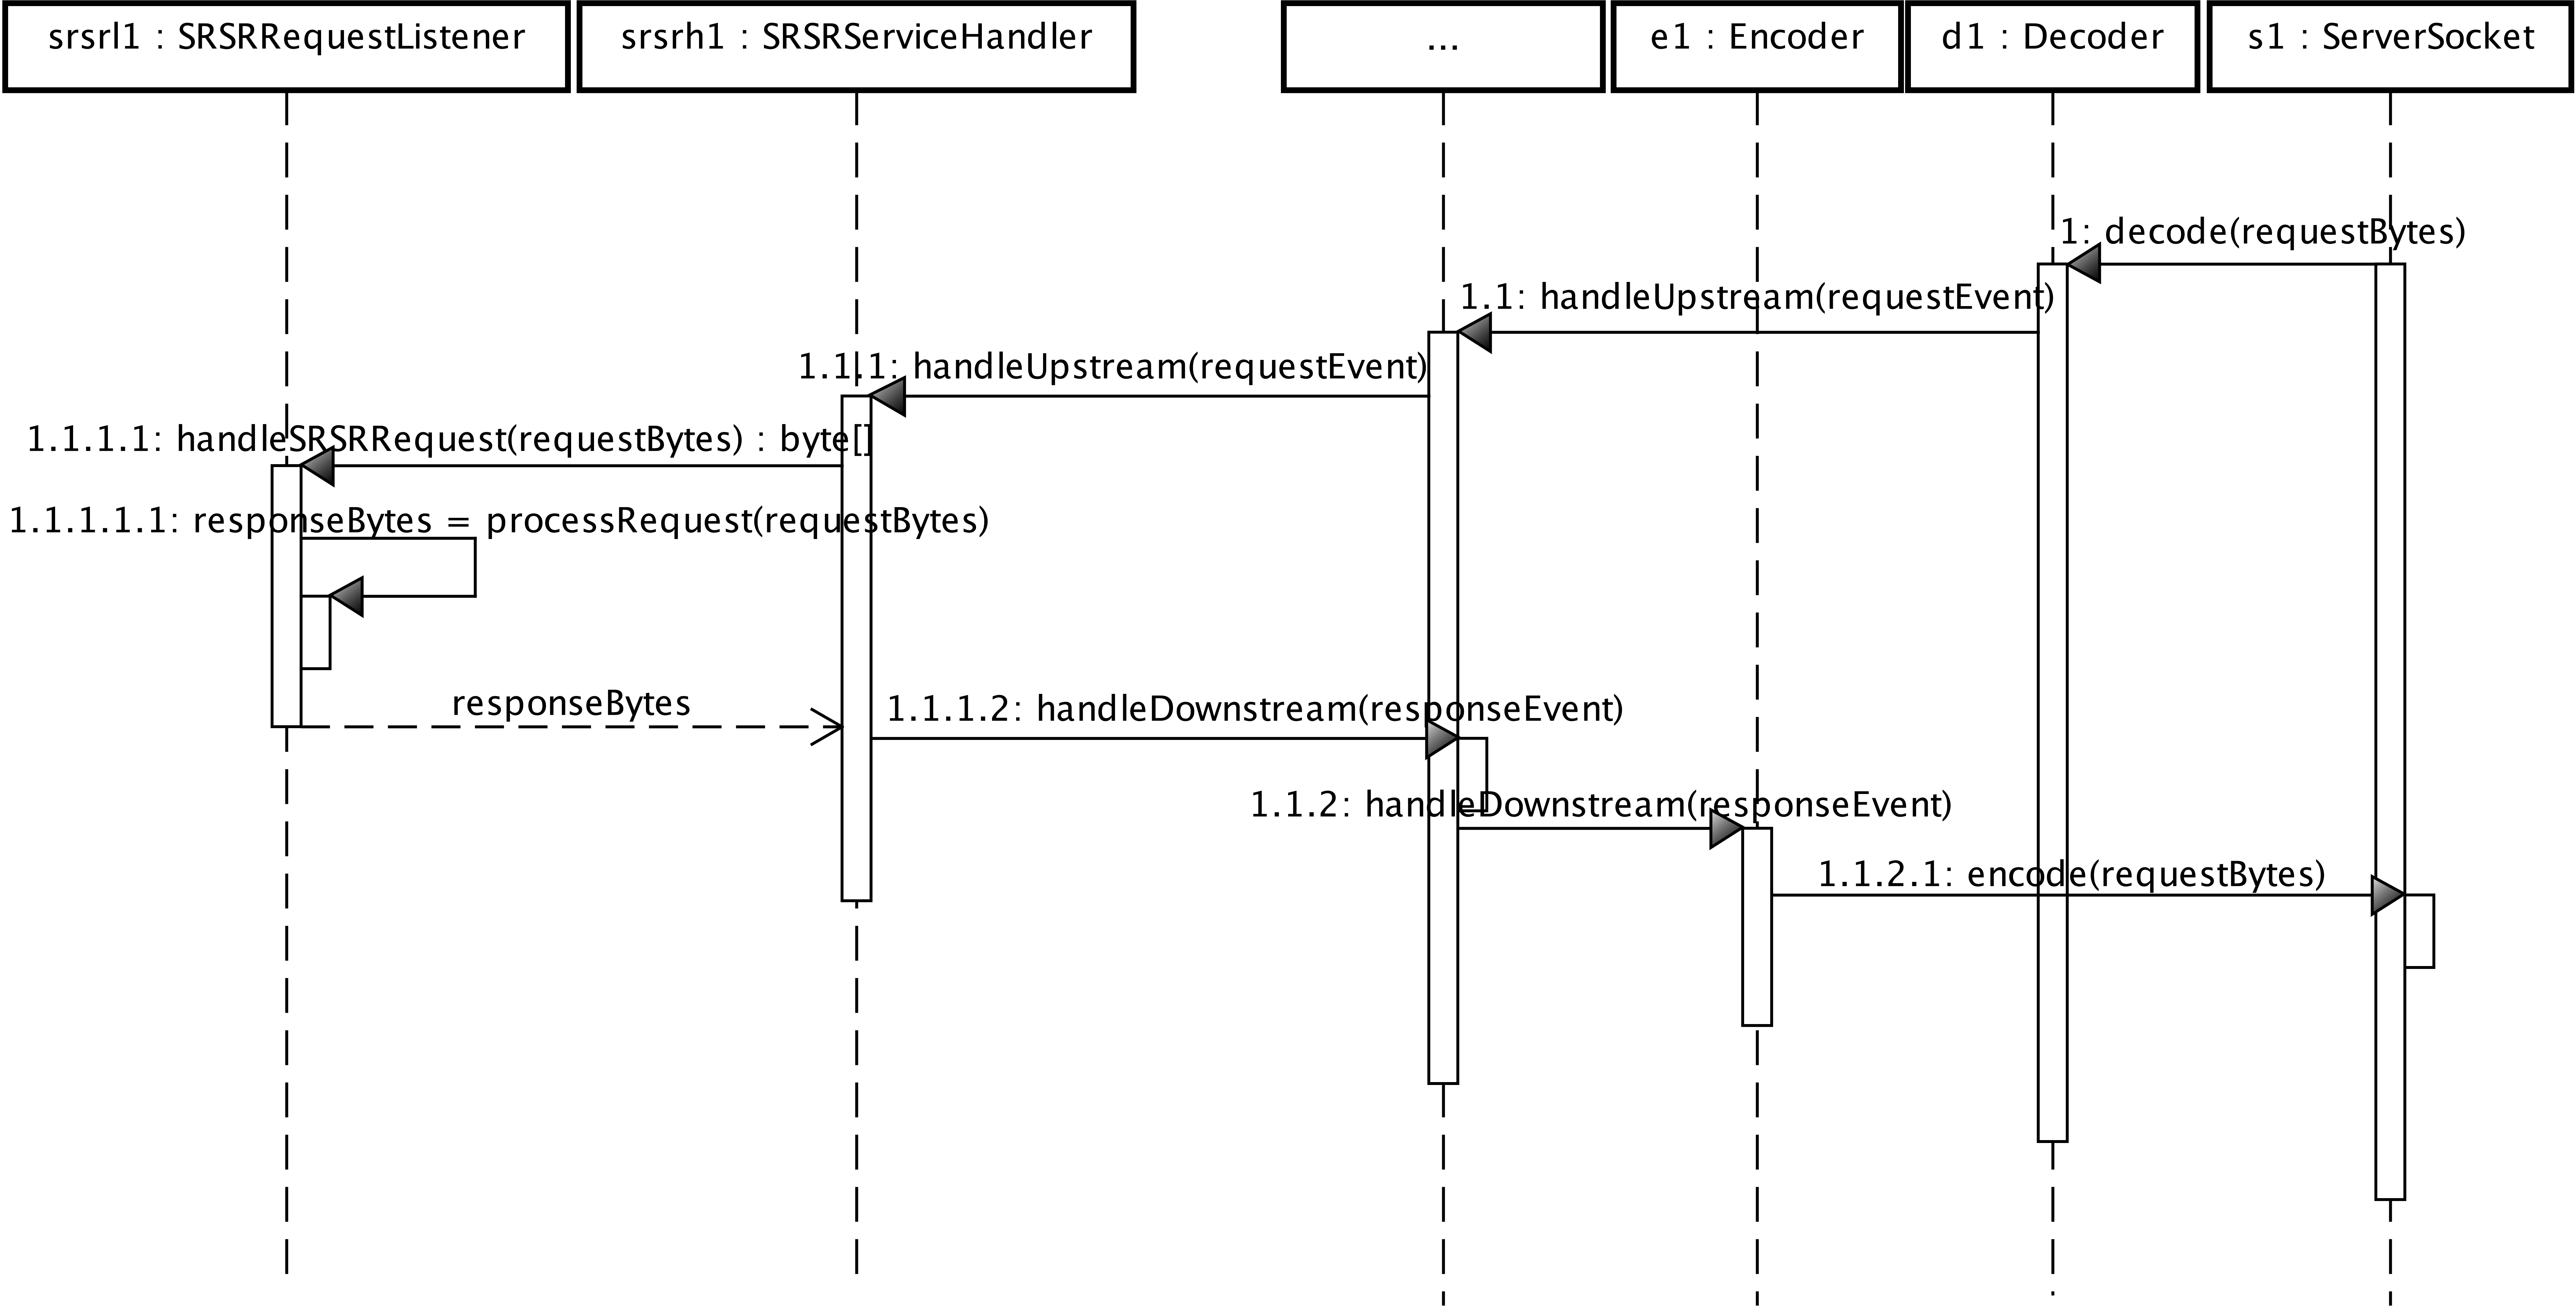
\includegraphics[width=12 cm]{img/sequence_srsr.png}
%\label{fig:sequence_srsr}
%\caption{Ablauf eines SingleRequestSingleResponse-Response}
%\end{figure}

\myfig{sequence_srsr}{sequenz}

Der Ablauf ist dabei wie folgt: Der Server-Socket liest bytes und reicht diese an den entsprechenden (Protobuf)-Decoder weiter. Dieser dekodiert die Nachricht und erzeugt daraus eine Protokoll-Nachricht. Diese wird als ChannelEvent upstream "uber die registrierten ChannelHandler an den SingleRequestSingleResponseServiceHandler weitergereicht. Der verantwortliche registrierte SingleRequestSingleResponseRequestListener bekommt den Payload "ubergeben, arbeitet den Request-Payload ab und gibt einen Response-Payload an den SingleRequestSingleResponseRequestListener zur"uck, der daraus eine korrespondierende Response-Protokoll-Nachricht erzeugt. Diese Nachricht wird dann "uber die Handler der Pipeline downstream zum (Protobuf-)Dekoder durchgereicht. Der Dekoder serialisiert die bytes und sendet diese an den Client-Socket zur"uck.

Der Ablauf f"ur die weiteren Nachrichtentypen des Message Exchange Pattern ist dabei analog, wobei sich jeweils nur der ServiceHandler und RequestListener ver"andert.

\subsubsection{RequestResponseChannel}
Wie bereits in der ChannelArchitektur im Abschnitt \ref{subsec:mep-arch-channel} des Entwurfskapitel beschrieben, besitzt Ubermep neben dem UnicastMulticastChannel eigene RequestResponseChannel, namentlich {\it SingleRequestSingleResponseChannel} bzw. {\it MultiResponseChannel}. Im Folgenden werden nun diese beiden Channels n"aher beschrieben. Das Zusammenspiel der verschiedenen Channels ist dabei in Abbildung \ref{fig:mep-app_srsr_mr_channel} veranschaulicht.

\paragraph{SingleRequestSingleResponseChannel} 
"Uber den SingleRequestSingleResponseChannel k"onnen ausschlie"slich SingleRequestSingleResponseRequests versendet werden. Dabei ist einzig die folgende Methode von Bedeutung:

\myfig[110mm]{mep-app_srsr_mr_channel}{Handling der RequestResponse-Events in Ubermep}

\begin{itemize}
\item {\it write(SingleRequestSingleResponseRequest request)} sendet einen SingleRequestSingleResponseRequest "uber den SingleRequestSingleResponseChannel. Der Response wird als Future-Objekt zur"uckgegeben. Eine genaue Beschreibung der zur"uckgelieferten Response findet sich weiter unten im Abschnitt \ref{subsec:ubermep_core_msg}.
\end{itemize}

\paragraph{MultiResponseChannel}"Uber den MultiResponseChannel k"onnen ausschlie"slich MultiResponseRequests, namentlich SingleRequestMultiResponseRequest bzw. MultiRequestMultiResponseRequest versendet werden. Dabei ist einzig die folgenden Methode von Bedeutung:

\begin{itemize}
\item {\it write(Request request)} sendet einen MultiResponseRequest "uber den MultiResponseChannel. Der Response wird als Future-Objekt zur"uckgegeben. Eine genaue Beschreibung der zur"uckgelieferten Response findet sich weiter unten im Abschnitt \ref{subsec:ubermep_core_msg}.
\end{itemize}

\subsubsection{UbermepRpcChannel}
Ubermep besitzt einen eigenen Channel f"ur den Aufruf von Remote Procedure Calls, den UbermepRpcChannel. Mittels diesem Channel k"onnen Stubs generiert werden, "uber die ein RPC aufgerufen werden kann. Die, f"ur den Aufruf entscheidenen Methoden, bezieht der UbermepRpcChannel aus dem Protobuf-Projekt. Die Abbildung \ref{fig:Dependencies_UbermepRpcChannel} veranschaulicht hierbei die Abh"angigkeiten. Die Methoden haben dabei die folgende Bedeutung:

\begin{itemize}
\item {\it callBlockingMethod(Descriptors.MethodDescriptor method, ...)} ruft einen blockierenden Remote Procedure Call auf und gibt die Antwort als Protokoll-Nachricht zur"uck. Blockierend bedeutet, das diese Methode solange den Aufrufer \emph{blockiert} bis eine Antwort empfangen wurde.
\item {\it callMethod(Descriptors.MethodDescriptor method, ...)} ruft einen nicht-blockierende Remote Procedure Call auf und gibt die Antwort als Protokoll-Nachricht in dem als Parameter "ubergebenen Callback zur"uck, wobei der Aufrufer hierbei \emph{nicht blockiert} wird.
\end{itemize}

\myfig{Dependencies_UbermepRpcChannel}{Abh"angigkeiten des UbermepRpcChannel}

\subsection{Messaging}
\label{subsec:ubermep_core_msg}
Im Folgenden Abschnitt werden nun die von Ubermep unterst"utzten Nachrichten-Pattern spezifiziert. Zuerst werden die Nachrichten des UnreliableMessaging-Pattern beschrieben danach die Nachrichten des ReliableMessaging.

In der nun folgenden Spezifikation haben dabei die verwendeten Eigenschaften die folgende Bedeutung:

\begin{itemize}
\item {\bf Parameter}: die der Nachricht zu "ubergebenen Parameter
\item {\bf PayloadListener}: der verantwortliche PayloadListener Server-seitig zum Lesen des Request-Inhalts und Schreiben des Response-Inhalts.
\item {\bf Response}: die zu erwartende Response bei erfolgreicher Auslieferung der Nachricht.
\item {\bf Optionale Parameter}: die der Nachricht optional zu "ubergebenen Parameter, wobei diese immer "uber entsprechende {\it Setter} gesetzt werden.
\item {\bf Erfolgreich ausgeliefert bei}: gibt an, wann eine Nachricht als \emph{erfolgreich ausgeliefert} gilt. Nur dann wird auch die entsprechende Response zur"uckgegeben.
\item {\bf ProgressListener}: das zu implementierende Interface Client-seitig.
\item {\bf Zur"uckgeliefert bei}: gibt an, wann eine Nachricht an den Sender zur"uckgeliefert wird.
\end{itemize}

\subsubsection{UnreliableRequest}
In diesem Abschnitt werden nun die Nachrichten des UnreliableMessaging-Pattern beschrieben.

\paragraph{UnreliableUnicastRequest}
Ein UnreliableUnicastRequest ist wie folgt spezifiziert:

%\begin{table}[h]
 %\caption{UnreliableUnicastRequest}
\begin{tabular}{|l|l|}
\hline 
{\bf Parameter} & remoteAddress : UPAddress \\
& payload : byte[] \\
\hline 
{\bf PayloadListener} & UnicastMulticastRequestListener (lesend) \\
\hline
{\bf Response} & keine \\
\hline
\end{tabular}
%\end{table}

\paragraph{UnreliableMulticastRequest}
Ein UnreliableMulticastRequest ist wie folgt spezifiziert:

%\begin{table}[h]
% \caption{UnreliableMulticastRequest}
\begin{tabular}{|l|l|}
\hline 
{\bf Parameter} & remoteAddresses : Collection$<$UPAddress$>$ \\
& payload : byte[] \\
\hline 
{\bf PayloadListener} & UnicastMulticastRequestListener (lesend) \\
\hline
{\bf Response} & keine \\
\hline
\end{tabular}
%\end{table}

\subsubsection{ReliableRequest}
In diesem Abschnitt werden die Nachrichten des ReliableMessaging-Pattern spezifiziert.

\paragraph{ReliableUnicastRequest}
Ein ReliableUnicastRequest ist wie folgt spezifiziert:

%\begin{table}[h]
% \caption{ReliableUnicastRequest}
\begin{tabular}{|l|l|}
\hline 
{\bf Parameter} & remoteAddress : UPAddress \\
& payload : byte[] \\
\hline
 {\bf optionale Parameter} & timeOut : int \\
 & timeOutUnit : TimeUnit \\
 \hline
 {\bf PayloadListener} & UnicastMulticastRequestListener (lesend) \\
 \hline
 {\bf Response} & ReliableUnicastResponse \\
 \hline
  {\bf Erfolgreich ausgeliefert bei} & Eingang der Nachricht am Empf"anger-Peer \\
  \hline
\end{tabular}
%\end{table}

\paragraph{ReliableMulticastRequest}
Ein ReliableMulticastRequest ist wie folgt spezifiziert:

%\begin{table}[h]
% \caption{ReliableMulticastRequest}
\begin{tabular}{|l|l|}
\hline 
{\bf Parameter} & remoteAddresses : Collection$<$UPAddress$>$ \\
& payload : byte[] \\
\hline
 {\bf optionale Parameter} & timeOut : int \\
 & timeOutUnit : TimeUnit \\
 \hline
 {\bf PayloadListener} & UnicastMulticastRequestListener (lesend) \\
 \hline
 {\bf Response} & ReliableMulticastResponse \\
 \hline
  {\bf Erfolgreich ausgeliefert bei} & Eingang der Nachricht am Empf"anger-Peer \\
  \hline
\end{tabular}
%\end{table}

Anmerkung: Eine ReliableMulticastResponse enth"alt die Responses als Map. Die Responses werden dabei in der Map-"ublichen Weise,  also als \emph{Key,Value}-Paar   
der Response-Map hinzugef"ugt. Der {\it Key} entspricht dabei der UPAddress des geantworteten Peers, der {\it Value} einer einzelnen Response vom Typ  {\it Reli\-ableMulticastResponse.SingleReliableMulticastResponse}.

\paragraph{SingleRequestSingleResponseRequest}
Ein SingleRequestSingleResponseRequest ist wie folgt spezifiziert:

%\begin{table}[h]
% \caption{SingleRequestSingleResponseRequest}
\begin{tabular}{|l|l|}
\hline 
{\bf Parameter} & remoteAddress : UPAddress \\
& payload : byte[] \\
\hline
 {\bf optionale Parameter} & timeOut : int \\
 & timeOutUnit : TimeUnit \\
 \hline
 {\bf PayloadListener} & SingleRequestSingleResponseRequestListener\\
 & (lesend und schreibend) \\
 \hline
 {\bf Response} & SingleRequestSingleResponseResponse \\
 \hline
  {\bf Erfolgreich ausgeliefert bei} & Eingang der Nachricht am Empf"anger-Peer {\bf und} \\
 & erfolgreicher Verarbeitung eines PayloadListener \\
  \hline
\end{tabular}
%\end{table}

\paragraph{SingleRequestMultiResponseRequest}
Ein SingleRequestMultiResponseRequest ist wie folgt spezifiziert:

%\begin{table}[h]
% \caption{SingleRequestMultiResponseRequest}
\begin{tabular}{|l|l|}
\hline 
{\bf Parameter} & remoteAddress : UPAddress \\
& payload : byte[] \\
\hline
 {\bf optionale Parameter} & timeOut : int \\
 & timeOutUnit : TimeUnit \\
 \hline
 {\bf PayloadListener} & MultiResponseRequestListener\\
 & (lesend und schreibend) \\
 \hline
  {\bf ProgressListener} & ProgressListenerRunnable \\
 \hline
 {\bf Response} & SingleRequestMultiResponseResponse \\
 \hline
  {\bf Erfolgreich ausgeliefert bei} & Eingang der Nachricht am Empf"anger-Peer {\bf und} \\
 & erfolgreicher Verarbeitung eines PayloadListener \\
  \hline
\end{tabular}
%\end{table}

%Anmerkung: Eine SingleRequestMultiResponse-Response enth"alt die Responses als Map. Die Responses werden dabei in der Map-"ublichen Weise,  also als \emph{Key,Value}-Paar   
%der Response-Map hinzugef"ugt. Der {\it Key} entspricht dabei der UPAddress des geantworteten Peers, der {\it Value} einer einzelnen Response vom Typ  {\it SingleMultiResponseResponse}.

\paragraph{MultiRequestMultiResponseRequest}
Ein MultiRequestMultiResponseRequest ist wie folgt spezifiziert:

%\begin{table}[h]
% \caption{MultiRequestMultiResponseRequest}
\begin{tabular}{|l|l|}
\hline 
{\bf Parameter} & remoteAddresses : Collection$<$UPAddress$>$ \\
& payload : byte[] \\
\hline
 {\bf optionale Parameter} & timeOut : int \\
 & timeOutUnit : TimeUnit \\
 \hline
 {\bf PayloadListener} & MultiResponseRequestListener\\
 & (lesend und schreibend) \\
 \hline
  {\bf ProgressListener} & ProgressListenerRunnable \\
 \hline
 {\bf Response} & MultiRequestMultiResponseResponse \\
 \hline
  {\bf Erfolgreich ausgeliefert bei} & Eingang der Nachricht am Empf"anger-Peer {\bf und} \\
 & erfolgreicher Verarbeitung eines PayloadListener \\
  \hline
\end{tabular}
%\end{table}

Anmerkung: Eine MultiResponse-Response enth"alt die Responses als Map. Die Responses werden dabei in der Map-"ublichen Weise,  also als \emph{Key,Value}-Paar   
der Response-Map hinzugef"ugt. Der {\it Key} entspricht dabei der UPAddress des geantworteten Peers, der {\it Value} einer einzelnen Response vom Typ  {\it SingleMultiResponseResponse}.

\subsubsection{ReliableResponse}
Einzig Nachrichten des oben beschriebenen ReliableMessaging-Pattern liefern Responses zur"uck. Dabei gibt es, wie oben spezifiziert, f"ur einen erfolgreich ausgelieferten ReliableRequest einen korrespondierenden ReliableResponse. Des weiteren gibt es f"ur diesen Request ReliableResponses bei \emph{nicht erfolgreicher} "Ubertragung. Im Folgenden werden nun diese beschrieben.

\paragraph{ErrorResponse}
Eine ErrorResponse ist wie folgt spezifiziert:

%\begin{table}[h]
% \caption{MultiRequestMultiResponseRequest}
\begin{tabular}{|l|l|}
\hline 
{\bf Parameter} & request : Request \\
& localAddress : UPAddress \\
& cause : Throwable \\
 \hline
  {\bf Zur"uckgeliefert bei} & Fehlerhafter "Ubertragung einer Nachricht \\
  \hline
\end{tabular}
%\end{table}

\paragraph{TimeOutResponse}
Eine TimeOutResponse ist wie folgt spezifiziert:

%\begin{table}[h]
% \caption{MultiRequestMultiResponseRequest}
\begin{tabular}{|l|l|}
\hline 
{\bf Parameter} & request : Request \\
& localAddress : UPAddress \\
 \hline
  {\bf Zur"uckgeliefert bei} & TimeOut w"ahrend der Auslieferung, ausgel"ost durch: \\
  & TimeOut des Request wenn gesetzt, \\
  & sonst DefaultTimeOut (siehe dazu Abschnitt \ref{subsec:ubermep-core_konfiguration} ) \\
  \hline
\end{tabular}
%\end{table}

\subsection{Konfiguration}
\label{subsec:ubermep-core_konfiguration}
Die Konfiguration von Ubermep erfolgt "uber das konfigurieren der einzelnen Peers des Netzwerks. Dies geschieht "uber Variablen der Klasse {\it PeerConfig}. Die nun folgenden Spezifikationen sind dabei wie folgt aufgebaut:

\paragraph{\{Variablenname\}}
\begin{itemize}
\item {\bf \{Verwendung\}}
\item {\bf \{Typ\}}
\item  {\bf \{DefaultValue\}}
\end{itemize}

\subsubsection{Konfiguration eines Peers}
Die Konfiguration eines Peers ist wie folgt spezifiziert: 

\paragraph{CORE\_POOL\_SIZE}
\begin{itemize}
\item {\bf Verwendung}: Die maximale Gr"o"se der von Uberlay verwendeten ThreadPools 
\item {\bf Typ}: int
\item  {\bf DefaultValue}: 10
\end{itemize}
	
\paragraph{DEFAULT\_TIMEOUT}
\begin{itemize}
\item {\bf Verwendung}: Die DefaultTimeOut f"ur ReliableRequests.
\item {\bf Typ}: int
\item  {\bf DefaultValue}: 30
\end{itemize}

\paragraph{DEFAULT\_TIMEOUT\_TIMEUNIT}
\begin{itemize}
\item {\bf Verwendung}: Die Default-Zeiteinheit der DEFAULT\_TIMEOUT
\item {\bf Typ}: TimeUnit
\item  {\bf DefaultValue}: TimeUnit.SECONDS
\end{itemize}

\paragraph{UberlayModule.RTT\_REQUEST\_INTERVAL}
\begin{itemize}
\item {\bf Verwendung}: Das Interval in dem die RoutingTabellen eines Peers mittels des RoundTripTime-Protokolls von Uberlay aktualisiert werden. (siehe dazu Abschnitt \ref{subsec:uberlay-rtt} im Grundlagenkapitel)
\item {\bf Typ}: int
\item  {\bf DefaultValue}: 10
\end{itemize}

\paragraph{UberlayModule.RTT\_REQUEST\_INTERVAL\_TIMEUNIT}
\begin{itemize}
\item {\bf Verwendung}: Die Default-Zeiteinheit des RTT\_REQUEST\_INTERVAL
\item {\bf Typ}: int
\item  {\bf DefaultValue}: TimeUnit.SECONDS
\end{itemize}

\section{Beispiele}
\label{sec:beispiele}
Im Folgenden soll nun anhand von Beispielen die Funktionalit"at von Ubermep veranschaulicht werden. Dazu wird ein kleines Peer-to-Peer Netzwerk mit 3 Knoten erzeugt, "uber die Nachrichten des Message Exchange Pattern versendet werden k"onnen. Die Abbildung \ref{fig:example_p2p_network} zeigt dabei den Aufbau des Netzwerks.

\subsection{Aufbau eines Peer-to-Peer Netzwerk}
Im nun folgenden Beispiel wird ein Peer-to-Peer Netzwerk wie folgt aufgebaut:

\myfig{example_p2p_network}{Aufbau eines einfachen Peer-to-Peer Netzwerk}

Der entsprechende Quellcode sieht dabei wie folgt aus:

\lstset{caption=Aufbau eines einfachen Peer-to-Peer Netzwerk,tabsize=4,language=Java,firstnumber=1, label=bsp:createPeer}
\begin{lstlisting}
// Peers erzeugen ... 
Peer server = new PeerImpl(new UPAddress("urn:itm:1"), 
	new InetSocketAddress("0.0.0.0", 8080));
Peer transitHost = new PeerImpl(new UPAddress("urn:itm:2"), 
	new InetSocketAddress("0.0.0.0", 8081), 
	new InetSocketAddress("0.0.0.0", 8080));
Peer client = new PeerImpl(new UPAddress("urn:itm:3"), 
	new InetSocketAddress("0.0.0.0", 8082), 
	new InetSocketAddress("0.0.0.0", 8081));

// Peers starten ...
server.start();
transitHost.start();
client.start();

// ... kommuniziere ein wenig ...

// Peers stoppen
client.stop();
transitHost.stop();
server.stop();
\end{lstlisting}

\subsection{Kommunikation}

\nomenclature{WSN}{Wireless Sensor Network}

Nachdem nun das Netzwerk aufgebaut ist, kann "uber die Knoten kommuniziert werden. In den nun folgenden Beispielen sollen Nachrichten erzeugt und versendet werden, um ausgew"ahlte Peers (Nodes) zu \emph{flashen}. \emph{Flashen} bedeutet hier: Das Aufspielen einer neuen Firmware auf einem Knoten. Diese Funktionalit"at spielt z.B. eine Rolle in {\it Wireless Sensor Networks (WSN's)}. Daf"ur werden in den folgenden Beispielen der String {\tt flashNode} als ByteArray "ubertragen und ausgewertet.

\subsubsection{Unreliable Messaging}
Um Unicast- bzw. Multicast-Requests f"ur das flashen von Nodes verarbeiten zu k"onnen, muss zuerst der entsprechende UnicastMulticastRequestListener wie folgt erzeugt werden, dabei sei angenommen das eine entsprechende Methode {\it flashNode()} mit der oben beschriebenen Funktionalit"at vorhanden ist:

\lstset{caption=Erzeugen eines UnicastMulticastRequestListener,tabsize=2,language=Java,firstnumber=1, label=bsp:createRequestListener}
\begin{lstlisting}
UnicastMulticastRequestListener flashNodeUnicastMulticastRequestListener = new UnicastMulticastRequestListener() {
	public boolean handleUnicastMulticastRequest(String senderUrn, byte[] payload) {
		if (new String(payload).equals("flashNode")) {
			// aufrufen von flashNode()
			flashNode();
			return true;
		} else {
			return false;
		}
	}
};
\end{lstlisting}

Nun muss noch der {\it flashNodeUnicastMulticastRequestListener} am entsprechenden Peer Server-seitig hinzugef"ugt werden.

\lstset{caption=Hinzuf"ugen eines UnicastMulticastRequestListener,tabsize=2,language=Java,firstnumber=1, label=bsp:addUnicastMulticastRequestListener}
\begin{lstlisting}
server.addRequestListener(flashNodeUnicastMulticastRequestListener);
\end{lstlisting}

\paragraph{UnreliableUnicastRequest}
Anschlie"send kann ein entsprechender Unreliable\-Unicast\-Request an den Server wie folgt versendet werden:

\lstset{caption=Senden eines UnreliableUnicastRequest,tabsize=2,language=Java,firstnumber=1, label=bsp:sendUnrelUnicast}
\begin{lstlisting}
UnreliableRequest request = new UnreliableUnicastRequest(server.getLocalUPAddress(), "flashNode".getBytes());
client.send(request);
\end{lstlisting}

\paragraph{UnreliableMulticastRequest} 
Der Aufruf eines UnreliableMulticastRequest erfolgt analog zu dem eines UnreliableUnicastRequest.
\lstset{caption=Senden eines UnreliableMulticastRequest,tabsize=2,language=Java,firstnumber=1, label=bsp:sendUnrelMulticast}
\begin{lstlisting}
List<UPAddress> urns = new ArrayList<UPAddress>() {{
	add(server.getLocalUPAddress());
	add(...);
}};

UnreliableRequest request = new UnreliableMulticastRequest(urns, "flashNode".getBytes());
client.send(request);
\end{lstlisting}

\subsubsection{Reliable Messaging}
Nachrichten des Reliable Messaging Patterns k"onnen als blockierende als auch als nicht-blockierende Aufrufe versendet werden. Im Folgenden Beispiel werden nun die beiden Aufrufe dargestellt:

\lstset{caption=Blockierender und nicht-blockierender Nachrichtenempfang,tabsize=2,language=Java,firstnumber=1, label=bsp:blockingNonBlockingResponse}
\begin{lstlisting}
final ListenableFuture<Response> responseFuture = client.send(request);

//blockierender Aufruf
Response response = responseFuture.get();

//nicht-blockierender Aufruf
responseFuture.addListener(new Runnable() {
	public void run() {
		Response response = responseFuture.get();
	}}, new ScheduledThreadPoolExecutor(1));
...
\end{lstlisting}

In den folgenden Beispielen werden zur Vereinfachung nur blockierende Aufrufe beschrieben.

\paragraph{ReliableUnicastRequest} 
Mit Hilfe eines ReliableUnicastRequest kann nun "uberpr"uft werden, ob die Methode {\it flashNode()} tats"achlich aufgerufen wurde.
\lstset{caption=Senden eines ReliableUnicastRequest als blockierender Aufruf,tabsize=2,language=Java,firstnumber=1, label=bsp:sendRelUnicast}
\begin{lstlisting}
ReliableRequest request = new ReliableUnicastRequest(server.getLocalUPAddress(), "flashNode".getBytes());
Future<Response> responseFuture = client.send(request);

Response response = responseFuture.get();
if (response instanceof ReliableUnicastResponse){
	// tu was mit Response
}
\end{lstlisting}

\paragraph{ReliableMulticastRequest}
Der Aufruf eines ReliableMulticastRequest geschieht analog zu dem eines ReliableUnicastRequest.
\lstset{caption=Senden eines ReliableMulticastRequest,tabsize=2,language=Java,firstnumber=1,literate={�}{{\"u}}1, label=bsp:sendRelMulticast}
\begin{lstlisting}
List<UPAddress> urns = new ArrayList<UPAddress>() {{
	add(transitHost.getLocalUPAddress());
	add(...);
}};

ReliableRequest request = new ReliableMulticastRequest(urns, "flashNode".getBytes());
Future<Response> responseFuture = client.send(request);

Response response = responseFuture.get();
// "uberpr�fe Responses ... �ber: response.getResponses()
\end{lstlisting}

\paragraph{SingleRequestSingleResponseRequest}
Um einen SingleRequest\-Single\-Response\-Request f"ur das flashen eines Nodes verarbeiten zu k"onnen, muss zuerst der entsprechende SingleRequestSingleResponseRequestListener Server-seitig wie folgt erzeugt und hinzugef"ugt werden, dabei sei auch hier angenommen, dass eine entsprechende Methode {\it flash\-Node()} mit der beschriebenen Funktionalit"at vorhanden ist:
\lstset{caption=Erstellen eines SingleRequestSingleResponseRequestListener,tabsize=2,language=Java,firstnumber=1, label=bsp:createSRSRRequestListener}
\begin{lstlisting}
SingleRequestSingleResponseRequestListener flashNodeSingleRequestSingleResponseRequestListener = new SingleRequestSingleResponseRequestListener() {
	public byte[] handleSingleRequestSingleResponseRequest(String senderUrn, byte[] payload) throws UbermepExceptionEvent {
		if (new String(payload).equals("flashNode")) {
			try {
				// aufrufen von flashNode()
				flashNode();
				return "flashNode: Done".getBytes();
			} catch (Exception e){
				throw 
					new UbermepSingleResponseExceptionEvent(e.getCause());
			}
		} else {
			return null;
		}
	}
};

server.addRequestListener(flashNodeSingleRequestSingleResponseRequestListener);
\end{lstlisting}

Anschlie"send kann nun mit Hilfe eines SingleRequestSingleResponseRequest "uberpr"uft werden, ob die Methode {\it flashNode()} tats"achlich aufgerufen wurde:
\lstset{caption=Senden eines SingleRequestSingleResponseRequest,tabsize=2,language=Java,firstnumber=1,literate={�}{{\"u}}1, label=bsp:sendSRSR}
\begin{lstlisting}
ReliableRequest request = new SingleRequestSingleResponseRequest(server.getLocalUPAddress(), "flashNode".getBytes());
Future<Response> responseFuture = client.send(request);

Response response = responseFuture.get();
if (response instanceof SingleRequestSingleResponseResponse){
	// tu was mit Response, z.B. payload �berpr�fen
}
\end{lstlisting}

\paragraph{SingleRequestMultiResponseRequest}
Um einen Multi\-Response\-Request f"ur das Flashen eines Nodes verarbeiten zu k"onnen, muss zuerst der entsprechende MultiResponseRequestListener Server-seitig wie folgt erzeugt und hinzugef"ugt werden, dabei sei auch hier angenommen, dass eine Methode {\it flash\-Node()} mit der bereits beschriebenen Funktionalit"at vorhanden ist, wobei die Methode hier den Fortschritt in Prozent als Integer-Wert zur"uckgibt:

\lstset{caption=Hinzuf"ugen eines MultiResponseRequestListener,tabsize=2,language=Java,firstnumber=1, label=bsp:createMRRequestListener}
\begin{lstlisting}
MultiResponseRequestListener flashNodeMultiResponseRequestListener = new MultiResponseRequestListener() {
	public boolean handleMultiResponseRequest(MultiResponseHandle responseHandle, String senderUrn, byte[] payload) throws UbermepExceptionEvent {
		if (new String(payload).equals("flashNode")) {
			// aufrufen von flashNode()
			int percentDone = flashNode();
			while(percentDone < 50){;}
			// wenn flashNode() zu 50% fertig
			responseHandle.handleSingleResponse("flashNode:50% done".getBytes(), 1, 2);
			while(percentDone < 100){;}
			// wenn flashNode() fertig
			responseHandle.handleSingleResponse("flashNode:100% done".getBytes(), 2, 2);
			return true;
		} else {
			return false;
		}
	}
};

server.addRequestListener(flashNodeMultiResponseRequestListener);
\end{lstlisting}

Anschlie"send kann mit Hilfe eines SingleRequestMultiResponseRequest "uberpr"uft werden, ob die Methode {\it flashNode()} tats"achlich aufgerufen wurde und wie der Fortschritt ist.
\lstset{caption=Senden eines SingleRequestMultiResponseRequest,tabsize=2,language=Java,firstnumber=1, label=bsp:sendSRMR}
\begin{lstlisting}
ReliableRequest request = new SingleRequestMultiResponseRequest(server.getLocalUPAddress(), "flashNode".getBytes());
Future<Response> responseFuture = client.send(request);

Response response = responseFuture.get();
if (response instanceof SingleRequestMultiResponseResponse){
	// �berpr�fe Responses ... �ber: response.getResponses()
}
\end{lstlisting}

Das Hinzuf"ugen eines ProgressListeners f"ur eine SingleRequestMultiResponse\-Request-Nachrichten ist weiter unten erkl"art.

\paragraph{MultiRequestMultiResponseRequest}
Der Aufruf eines MultiRequestMultiResponseRequest geschieht analog zu dem eines SingleRequestMultiResponseRequest.
\lstset{caption=Senden eines MultiRequestMultiResponseRequest,tabsize=2,language=Java,firstnumber=1, label=bsp:sendMRMR}
\begin{lstlisting}
List<UPAddress> urns = new ArrayList<UPAddress>() {{
	add(server.getLocalUPAddress());
	add(...);
}};

ReliableRequest request = new MultiRequestMultiResponseRequest(urns, "flashNode".getBytes());
Future<Response> responseFuture = client.send(request);

//auf Response warten
Response response = responseFuture.get();
if (response instanceof MultiRequestMultiResponseResponse){
	// "uberpr�fe Responses ... �ber: response.getResponses()
}
\end{lstlisting}

Ein ProgressListener f"ur MultiResponse-Nachrichten l"a"st sich wie folgt Client-seitig hinzuf"ugen:

\lstset{caption=Verwenden eines ProgressListener,tabsize=2,language=Java,firstnumber=1, label=bsp:createProgressListener}
\begin{lstlisting}
//erzeuge ProgressListenerRunnable
ProgressListenerRunnable progressListenerRunnable = new ProgressListenerRunnable() {
	public void progress(String senderUrn, byte[] payload, int current, int total) {
		//tu etwas mit einzeln empfangener Response z.B. 
		log.info("received: " + current + " of " + total);
	}

	public void run() {
		//tu etwas mit komplett empfangener MultiResponse z.B. 
		Response response = responseFuture.get();
	}
};

// ProgressListener dem ResponseFuture hinzuf�gen
responseFuture.addListener(progressListenerRunnable, new ScheduledThreadPoolExecutor(2));
\end{lstlisting}


\subsubsection{RPC}
In dem folgenden Beispiel soll veranschaulicht werden, wie Remote Procedure Calls in Ubermep aufgerufen werden k"onnen. Dies wird mittels der bereits beschriebenen  Funktionalit"at des flashens von Nodes veranschaulicht. Dazu mu"s zuerst mittels der Protobuf-IDL (siehe Abschnitt \ref{sec:google-protobuf} im Grundlagenkapitel) ein \emph{FlashNodeServiceProtokoll} erzeugt werden. Das Listing \ref{lst:ubermep_flash_node_rpc} zeigt daf"ur ein Beispiel-Protokoll, welches anschlie"send mittels des protoc-Compiler in eine Java-Klasse "ubersetzt wird. Der Aufruf der Methode \emph{flashNode} erfolgt dabei "uber ein FlashNodeRequest, welcher einen Parameter {\it delay} enth"alt. Das Ergebnis des Aufrufs wird "uber den FlashNodeResponse zur"uckgegeben, wobei daf"ur ein Parameter {\it success} hinzugef"ugt wurde.

\lstinputlisting[language=Python,label=lst:ubermep_flash_node_rpc,caption=FlashNodeServiceProtocol.proto]{lst/FlashNodeServiceProtocol.proto}

Anschlie"send wird eine Implementierung des Service-Interface erzeugt, wobei im Folgenden Beispiel eine Implementierung des BlockingInterface verwendet wurde. 
Im Folgenden sei auch hier angenommen, dass eine Methode {\it flash\-Node()} mit der bereits beschriebenen Funktionalit"at vorhanden ist ,wobei die Methode hier als Parameter einen {\it delay} als Verz"ogerung des Aufrufs "ubergeben bekommt.

\lstset{caption=Implementierung des FlashNodeBlockingService,tabsize=2,language=Java,firstnumber=1, label=bsp:createBlockingService}
\begin{lstlisting}
public class FlashNodeBlockingServiceImpl implements FlashNodeServiceProtocol.FlashNodeService.BlockingInterface, RpcBlockingService{
	@Override
	public FlashNodeServiceProtocol.FlashNodeResponse flashNode(RpcController controller, FlashNodeServiceProtocol.FlashNodeRequest request) throws ServiceException {
		// aufrufen von flashNode(delay)
		flashNode(request.getDelay());
		return FlashNodeServiceProtocol.FlashNodeResponse.newBuilder().setSuccess(true).build();
	}

	@Override
	public BlockingService getRpcBlockingService() {
		return FlashNodeServiceProtocol.FlashNodeService.newReflectiveBlockingService(this);
	}
}
\end{lstlisting}
Im Folgenden soll nun ein RPC, "uber das bereits oben erzeugte Peer-to-Peer Netzwerk, vom Client auf dem Server ausgef"uhrt werden. Hierf"ur muss zuerst die {\it FlashNodeBlockingServiceImpl} am entsprechenden Peer Server-seitig hinzugef"ugt werden. Anschlie"send kann ein entsprechender FlashNodeRequest mit\-tels des RPC-Channel auf dem Server wie folgt aufgerufen werden:
\lstset{caption=Aufruf des FlashNodeBlockingService,tabsize=2,language=Java,firstnumber=1,literate={�}{{\"u}}1, label=bsp:callBlockingService}
\begin{lstlisting}
//Service am Server registrieren
server.registerService(new FlashNodeBlockingServiceImpl());

// erzeuge RPC-Request mit delay=10
FlashNodeServiceProtocol.FlashNodeRequest request = FlashNodeServiceProtocol.FlashNodeRequest.newBuilder().setDelay(10).build();

// hole RPC-Channel
UbermepRpcChannel blockingServerRpcChannel = client.getRpcChannel(blockingServerUrn);
// erzeuge neuen Blocking-Stub f�r FlashNodeService mittels RPC-Channel
FlashNodeServiceProtocol.FlashNodeService.BlockingInterface blockingService = FlashNodeServiceProtocol.FlashNodeService.newBlockingStub(blockingServerRpcChannel);

try {
	//rufe flashNodeService auf
	FlashNodeServiceProtocol.FlashNodeResponse rpcResponse = blockingService.flashNode(new RpcControllerImpl(), request);

	// tu was mit RPC-Response, z.B. success �berpr�fen	
} catch (ServiceException e) {
	// tu was mit ServiceException
}
\end{lstlisting}

Der Aufruf eines (non-blocking)-Service ist analog und soll deshalb hier nicht weiter vertieft werden. Nur soviel: der Service-Aufruf ben"otigt eine zus"atzliche (non-blocking)-Service-Implementierung sowie einen Callback, der aber einfach "uber:
\lstset{caption=Erzeugung eines FlashNodeServiceCallback,tabsize=2,language=Java,firstnumber=1,literate={�}{{\"u}}1, label=bsp:createServiceCallback}
\begin{lstlisting}
MEPRpcCallback<FlashNodeServiceProtocol.FlashNodeResponse> callback = new RpcCallbackImpl<FlashNodeServiceProtocol.FlashNodeResponse>();
\end{lstlisting}
erzeugt werden kann.

%\section{Zuk"unftige Erweiterungen}
%\label{sec:zukunft}

%Folgende Erweiterungen sind fest f"ur die n"ahere Zukunft eingeplant:
%\begin{itemize}
%\item Entwurf und die Implementierung des Publish-Subscribe Pattern zur Unterst"utzung von Publish-Subscribe ... f"ur Peers.
%\item Hinzuf"ugen einer Peer-to-Peer-Proxy-Funktionalit"at und daraus resultierend auch das Hinzuf"ugen einer Firewall-Funktionalit"at f"ur bestimmte Peers zum Kontrollieren von deren Netzwerkverkehr.
%\item Erweiterung des RoundTripTime-Protokoll von Uberlay um eine dynamische Anpassung der Zeitintervalle, z.B. mittels einer Implementierung des {\it Trickle}-Algorithmus \cite{trickle}.
%\end{itemize} 